%%
% The BIThesis Template for Bachelor Graduation Thesis
%
% 北京理工大学毕业设计(论文)第一章节 —— 使用 XeLaTeX 编译
%
% Copyright 2020 Spencer Woo
%
% This work may be distributed and/or modified under the
% conditions of the LaTeX Project Public License, either version 1.3
% of this license or (at your option) any later version.
% The latest version of this license is in
%   http://www.latex-project.org/lppl.txt
% and version 1.3 or later is part of all distributions of LaTeX
% version 2005/12/01 or later.
%
% This work has the LPPL maintenance status `maintained'.
%
% The Current Maintainer of this work is Spencer Woo.
%
% 第一章节

\chapter{前言}

\section{系统背景}
奖学金是教务、教学系统中的重要组成部分,对奖学金进行推荐与效果评估对教学管理与学生发展都有重要意义,这其中主要包括两部分的内容:分别是奖学金分配与奖学金评价,在此我将分别进行介绍。

第一部分是如何进行奖学金分配,即以奖学金的规定为标准对奖学金进行分发,我们有两种手段,一种是根据现有的标准对学生的多种指标(成绩、论文、竞赛等)进行数值换算从而得到数值评价并直接按数值顺序等规则颁发奖学金,也就是现在在本科生奖学金颁发中常用的综合测评等评价指标,这种方法主要基于已有的经验公式进行奖学金计算与推荐;第二种则是以学生的获奖、论文、竞赛等为依据以奖学金申请条件为标准进行推荐,这种方法是以推荐系统的思想为基础进行推荐,但是这种推荐与常用的内容、商品推荐等亦有差别,主要体现为内容、商品等信息推荐能够通过用户在平台积累的大量历史数据信息获得较为完整的用户画像,并且平台累积的用户数据丰富,适合进行推荐,而本研究的系统数据量少而且标签分布不均匀,对推荐算法的设计与特征的构建而言是一个较大的困难与挑战。

第二部分是通过学生的历史奖学金记录与其获奖周边历史信息对奖学金效果进行评价,这里就需要对用户进行时序上的画像,那么如何构建评价指标也是比较困难的一个工作,因为衡量效果的指标有多种,包括成绩变化、论文发表、专利申请、竞赛获奖等内容,需要对评价指标进行设计,而这仅仅是数据的标签部分,甚至于数据的标签可能是一个向量输出多维度指标也有可能,训练的特征也需要进行设计才能使模型进行有效的评价,这里可能需要用到时序的神经网络才能实现。这一部分由于本研究的数据量过少且分布不均匀而没有进行实现。所以可以看到在奖学金这个领域相关研究基本处于空白状态。

我同时查询了与奖学金有关的推荐系统,在这个领域基本处于空白状态,与此类似的系统绝大部分集中于对应届生进行工作推荐,如大学生兼职电商平台工作推荐系统的实现\cite{郭洁畅2017大学生兼职电商平台工作推荐系统的实现}、一种面向冷启动学生用户的工作推荐系统及推荐方法\cite{一种面向冷启动学生用户的工作推荐系统及推荐方法}等。国外的相关文献绝大部分也集中于对教学资源的分配与推荐,如EduRecomSys: An Educational Resource Recommender System Based on Collaborative Filtering and Emotion Detection\cite{bustos2020edurecomsys}。

可以看到在奖学金推荐这个领域相关研究基本处于空白状态。

\section{类似系统现状及问题}

推荐的基础是数据,对于一个典型的推荐系统而言,我们可以获得的数据总体来分为三种,分别是用户的信息、物品的信息以及用户的行为信息。所以按照数据来源可以将推荐系统分为基于内容的推荐以及基于用户行为的推荐两类。

总体而言,推荐系统的两大任务可以分为推荐和预测,所以推荐系统实现的评价指标也可以从上述两方面定义,分别是评分预测以及Top-N推荐,评分预测的目的就是通过已有的用户评价数据或者用户浏览数据对用户的评价模型进行学习;Top-N推荐是给用户推送一个根据用户浏览历史或者相似度信息匹配得到的包含多个内容项的以推荐列表形式呈现的信息。在我们的系统中我们主要希望实现的是Top-N推荐,从目前已有的数据来看共10种奖学金,系统预期的功能是给目标用户返回一个奖学金列表以提高推荐的成功率,降低用户手工对奖学金进行选择的时间成本,提高奖学金推送的推送效率。

Top-N推荐算法典型的应用场景为商品推荐系统,这也是目前研究、应用比较丰富的一类系统,在Amazon、豆瓣、淘宝、当当等电商、网商平台都有大规模的应用。此类系统中大致有两种思路,一种是基于商品把商品推荐给用户,也就对应于上文中基于内容的推荐,第二种是以用户为基础通过计算用户的相似性将用户推荐给商品,对应于上文中基于人口统计学和用户行为规则的推荐。图\ref{NetEase_Music}即为典型的Top-N个性化推荐系统。

\begin{figure}[htbp]
    \vspace{3pt} % 调整图片与上文的垂直距离
    \centering
    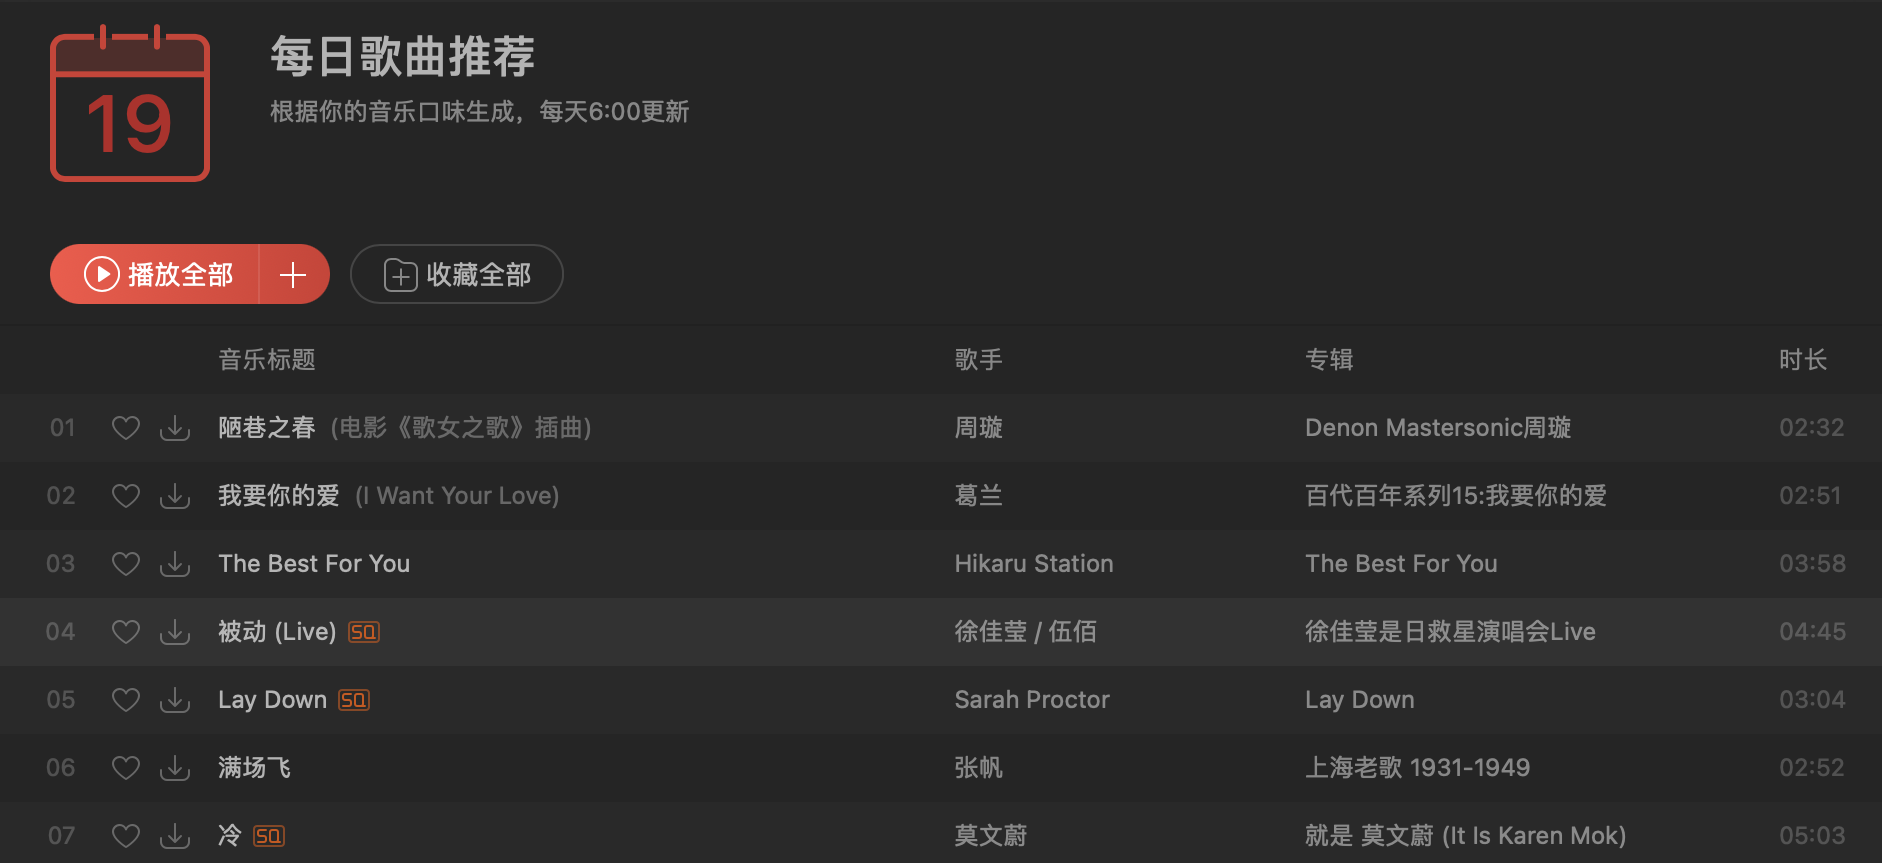
\includegraphics[width=0.9\textwidth]{images/NetEaseMusic.png}
    \caption{网易云音乐歌曲Top-N推荐}\label{NetEase_Music} % label 用来在文中索引
  \end{figure}

Top-N推荐的主要方法包括协同过滤算法(CF)、矩阵分解、因子分解机(Factorization Machines)、逻辑回归、梯度提升决策树(GBDT)、深度神经网络等为代表的一系列模型.

\subsection{传统机器学习模型}

在上述模型中基于协同过滤的推荐(Collaborative Filtering)\cite{su2009survey}算法是应用最早和最为成功的技术之一,协同过滤一般分为两大类,分别是基于近邻关系的过滤(neighborhood-based)和基于模型的过滤(model-based)。
其中基于近邻的过滤又可以分为两大类,分别是User-based与Item-based,这两类的区别在于基于用户的过滤\cite{荣辉桂2014基于用户相似度的协同过滤推荐算法}原理是利用用户的历史喜好信息计算用户之间的距离,然后利用相似用户的加权商品评分来对目标用户可能的购买行为进行预测,它能够有效的在较少的用户反馈量当中个性化学习其他相似用户的反馈信息\cite{姜保庆2014基于社交网络的一种个性化推荐算法}。

而Item-based\cite{deshpande2004item}的思想为通过计算商品和商品之间的相似度特征获取商品和商品之间的关联矩阵,通过对相似度高的商品进行预测目标用户评分得到用户的购买可能率。在最近邻的加权计算过程与相似度计算过程中,只分析了用户对用户或物品对物品的关系,所以它的运算速度相当快,并且在大型或小型的推荐系统都适用;而基于模型过滤则是最为常见的过滤算法类型,其原理是因为用户存在行为矩阵,用户的行为矩阵与物品之间存在隐变量,算法使用用户行为矩阵经过矩阵分解计算后的低阶用户矩阵和物品矩阵相乘来进行结果预测,其主流方法包括关联、聚类、分类、矩阵分解、神经网络及隐语义模型等。此类模型的推荐效果相对最近邻较好,但是算法训练时间较长复杂度较高使得推荐系统的训练以及在线推荐时间大幅上涨。由于基于模型的原理是用户和物品之间存在隐变量,所以早期推荐系统为了减少运算规模,常用推荐方法还有基于关联规则的推荐,由于用户的购买是存在关联性特征的,所以此类方法的主要思想就是通过算法统计用户的购买倾向,如对购买了商品集合A的用户和商品集合A与商品集合B存在关联的规则对用户推荐集合B中的商品。对于小型的推荐系统而言,使用较多的算法为Item-based的协同过滤算法,而对于大型的系统,由于存在丰富的用户特征以及商品特征,则可以考虑基于用户的协同过滤或基于模型的过滤算法。

但是随着数据量的积累,常用的数据特征工程方法one-hot encoding在面对大规模数据集的时候表现出了难以解决的缺陷,比如在一个有10000商品和1000000用户的系统中如果对用户的商品购买特点进行one-hot encoding那么总的特征空间过大而导致最终的特征矩阵过于稀疏,所以这样对网络的训练而言造成了比较大的困难,而且也导致了很多不必要的存储空间的浪费,所以大数据的高效处理也是一个棘手的问题。对于巨大的特征空间而言,可采用的方法包括使用PCA进行主成分分析降低特征维度,而且在实际应用中one-hot encoding后得到特征向量再经过PCA主成分分析进行降维的组合非常有用。除此以外FM、FFM以及DeepFM等也在此领域大显身手。

\subsection{深度学习模型}

神经网络、机器学习技术的进步协同过滤也有了一些新的思路,其中较为典型的思路包括使用GBDT或XGBoost等集成学习模型进行混合推荐、使用矩阵分解的思路对矩阵进行更快速的降维处理与提取、基于深度学习的协同过滤算法等。

随着深度神经网络在近年的发展,越来越多的模型也选择采用神经网络作为推荐算法进行推荐,典型的算法包括DeepFM、Wide \& Deep等,2016年Google提出的Wide \& Deep模型就在YouTube的视频推荐中应用并且取得了不凡的效果,
离线和在线测试相比传统的算法均有较大提高,同时2017年华为联合高校提出了DeepFM的方法,克服了Wide \& Deep需要手工特征工程的缺点结合FM和Wide \& Deep的优点对低阶和高阶特征同时进行学习,训练了一个使用FM+DNN的端到端神经网络。

但是协同过滤算法也包括一些固有的问题,比如典型的冷启动问题与特征空间稀疏问题。这两类问题目前都没有比较好的解决思路。其中冷启动问题在我们的实验数据上也会涉及。但是由于此系统的用户数据量比较少,对应的奖学金(商品)数量也比较少,所以这个问题同样无法适用于常见的冷启动解决思路。

\section{本文主要系统实现}

本文系统主要实现的是基于系统过滤的奖学金推荐算法,数据集来自计算机学院2016级学生以及2017级学生的真实数据,数据集中可用数据的规模在200人左右。在本文中首先进行了数据库架构的构建,然后将保存数据的excel文件转换为sqlite数据库当中的记录,再根据sqlite的记录进行筛选构建特征矩阵,而后用不同的协同过滤算法进行推荐系统的评估与构建。

在此系统实现后,其包含的机器学习算法也可以给其他类似的问题提供思路,比如教务系统中助学金的推荐、学生成绩预测等。在未来随着数据量的扩充可以结合Top-N推荐的思路对模型进行修改以满足多分类的需求。同时由于数据库使用的Django框架的ORM映射,所以可以通过搭建Django的apps实现可视化操作。

目前而言这个系统的主要难点在于如何进行用户特征的提取,由于数据规模较小可用的评价指标维度也相对不算丰富,所以对模型以及推荐的算法构成了较大的挑战。在本文中将分别对实验模型中出现的优化函数、目标函数、聚类算法、协同过滤算法等进行介绍。本文在特征构建处采用了一种特征融合方法,通过XGBoost将低维与高维特征进行融合,同时采用了多种不同的机器学习算法进行推荐;除了使用传统的机器学习算法外,本文也应用DeepFM进行了实验。

